
\section{Modelo de información de In-Help}

\subsection{Descripción general}
 En la figura~\ref{fig:Modelo_Info_In-Help} se muestra la estructura de información que manejará para la implementación del sistema y aplicación In-Help
 
\begin{figure}[htbp!]
	\begin{center}
		\fbox{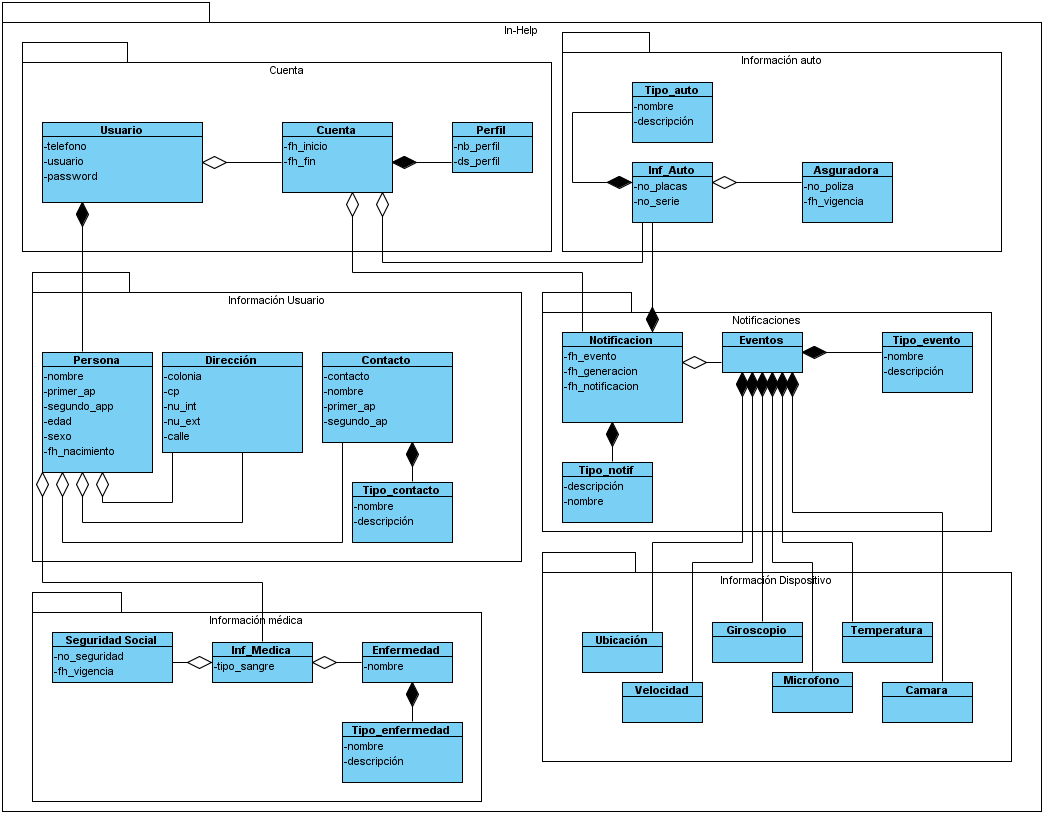
\includegraphics[width=1.1\textwidth]{ModeloNegocios/images/Informacion/DG_Informacion}}
		\caption{Modelo de información In-Help}
		\label{fig:Modelo_Info_In-Help}
	\end{center}
\end{figure}

\begin{BusinessEntity}{Usuario}{Usuario} 
    \Battr{usuario}{Usuario}{\tdCadena}{Es el identificador único para el usuario}{\requerido}{\longitudMinMax{5}{}{30}{}}
    \Battr{password}{Password}{\tdCadena}{Es la clave de acceso del usuario para la aplicación}{\requerido}{\longitudMinMax{8}{}{20}{}}
	\Battr{telefono}{Teléfono}{\tdNumerico}{Es el número de teléfono celular del usuario}{\requerido}{\longitudExacta{10}{}}
\end{BusinessEntity}

\begin{BusinessEntity}{Cuenta}{Cuenta} 
	\Battr{fh_inicio}{Fecha inicio}{\tdFecha}{Es la fecha en la que el usuario creo su cuenta}{\requerido}
	\Battr{fh_fin}{Fecha fin}{\tdFecha}{Es la fecha en la que el usuario elimino su cuenta}{\opcional}
\end{BusinessEntity}

\begin{BusinessEntity}{Perfil}{Perfil} 
	\Battr{nb_perfil}{Nombre de perfil}{\tdPalabra}{Es el nombre que identifica al perfil}{\requerido}{\longitudMinMax{2}{}{30}{}}
	\Battr{ds_perfil}{Descripción}{\tdFrase}{Es la descripción de perfil}{\requerido}{\longitudMinMax{10}{}{100}{}}

\end{BusinessEntity}

\begin{BusinessEntity}{Auto}{Auto} 
	\Battr{no_placas}{Placas}{\tdCadena}{Es uno de los identificadores únicos para el vehículo}{\requerido}{\longitudMinMax{6}{}{7}{}}
	\Battr{no_placas}{Serie}{\tdCadena}{Es el identificador único para el vehículo}{\opcional}{\longitudExacta{17}{}}
\end{BusinessEntity}

\begin{BusinessEntity}{TipoAuto}{Tipo de Auto} 
	\Battr{nb_perfil}{Nombre de perfil}{\tdCatalogo}{Es el \cdtRef{gls:TipoAuto}{tipo de automóvil}}{\requerido}
	
	\Battr{ds_tipo_auto}{Descripción}{\tdFrase}{Es la descripción de \cdtRef{gls:TipoAuto}{tipo de automóvil}
	}{\requerido}{\longitudMinMax{10}{}{100}{}}
\end{BusinessEntity}

\begin{BusinessEntity}{Aseguradora}{Aseguradora} 
	\Battr{no_poliza}{Póliza}{\tdCadena}{Es el número de poliza de seguro del automóvil}{\opcional}{\longitudMinMax{5}{}{30}{}}
	\Battr{fh_vigencia}{Vigencia}{\tdFecha}{Es la fecha de vigencia de la póliza de seguro del vehículo}{\opcional}
	
\end{BusinessEntity}


\begin{BusinessEntity}{Persona}{Persona} 
	\Battr{nombre}{Nombre}{\tdCadena}{Es el nombre de pila de la persona}{\requerido}{\longitudMinMax{5}{}{30}{}}
	\Battr{pri_ape}{Primer apellido}{\tdCadena}{Es el primer apellido de la persona}{\requerido}{\longitudMinMax{5}{}{30}{}}
	\Battr{seg_ape}{Segundo apellido}{\tdCadena}{Es el segundo apellido de la persona}{\opcional}{\longitudMinMax{5}{}{30}{}}
	\Battr{edad}{Edad}{\tdNumerico}{Es la edad de la persona}{\requerido}
	\Battr{sexo}{Sexo}{\tdCatalogo}{Es el \cdtRef{gls:sexo}{sexo} de la persona}{\requerido}
	\Battr{fh_nacimiento}{Fecha de nacimiento}{\tdFecha}{Es la fecha de nacimiento de la persona}{\opcional}
\end{BusinessEntity}

\begin{BusinessEntity}{Direccion}{Dirección} 
	\Battr{colonia}{Colonia}{\tdCadena}{Es el nombre de la colonia del domicilio de la persona}{\opcional}{\longitudMinMax{5}{}{30}{}}
	\Battr{cp}{Código Postal}{\tdNumerico}{Es la edad de la persona}{\opcional}
	\Battr{no_int}{Número interior}{\tdNumerico}{Es el número interior del domicilio de la persona}{\opcional}
	\Battr{no_ext}{Número exterior}{\tdNumerico}{Es el número exterior del domicilio de la persona}{\opcional}
	\Battr{calle}{Calle}{\tdCadena}{Es el nombre de la calle del domicilio de la persona}{\opcional}{\longitudMinMax{5}{}{30}{}}
\end{BusinessEntity}

\begin{BusinessEntity}{Contacto}{Contacto}
	\Battr{nombrec}{Nombre}{\tdCadena}{Es el nombre de pila del contacto}{\opcional}{\longitudMinMax{5}{}{30}{}}
	\Battr{pri_apec}{Primer apellido}{\tdCadena}{Es el primer apellido del contacto}{\opcional}{\longitudMinMax{5}{}{30}{}}
	\Battr{seg_apec}{Segundo apellido}{\tdCadena}{Es el segundo apellido del contacto}{\opcional}{\longitudMinMax{5}{}{30}{}}
	\Battr{telefonoc}{Teléfono}{\tdNumerico}{Es el número de teléfono del contacto}{\requerido}{\longitudExacta{10}{}}
\end{BusinessEntity}


\begin{BusinessEntity}{TipoContacto}{Tipo de Contacto} 
	\Battr{nb_contacto}{Nombre}{\tdCatalogo}{Es el \cdtRef{gls:TipoContacto}{tipo de contacto}}{\requerido}
	
	\Battr{ds_tipo_contacto}{Descripción}{\tdFrase}{Es la descripción de \cdtRef{gls:TipoContacto}{tipo de contacto}
	}{\requerido}{\longitudMinMax{10}{}{100}{}}
\end{BusinessEntity}

\begin{BusinessEntity}{Notificacion}{Notificación} 
	\Battr{fh_evento}{Fecha de evento}{\tdFecha}{Es la fecha en la que se registro el percanse}{\requerido}
	\Battr{fh_generación}{Fecha generación}{\tdFecha}{Es la fecha en la que se genero la notificación}{\opcional}
	\Battr{fh_notificacion}{Fecha notificación}{\tdFecha}{Es la fecha en la que se envió la notificación}{\opcional}
\end{BusinessEntity}

\begin{BusinessEntity}{TipNotif}{Tipo de Notificación} 
	\Battr{nb_noti}{Nombre}{\tdCatalogo}{Es el \cdtRef{gls:TipoNotificacion}{tipo de notificación}}{\requerido}
	
	\Battr{ds_nb_noti}{Descripción}{\tdFrase}{Es la descripción de \cdtRef{gls:TipoNotificacion}{tipo de notificación}
	}{\requerido}{\longitudMinMax{10}{}{100}{}}
\end{BusinessEntity}

\begin{BusinessEntity}{Eventos}{Eventos} 
	\Battr{nb_evento}{Nombre}{\tdCadena}{Es el evento que se registro}{\requerido}{}
\end{BusinessEntity}

\begin{BusinessEntity}{SeguridadSocial}{Seguridad Social} 
	\Battr{no_seguridad}{Número de seguridad}{\tdCadena}{Es el número de seguridad social del usuario}{\opcional}{\longitudMinMax{6}{}{30}{}}
	\Battr{fh_vegencia_seguridad}{Fecha de vigencia}{\tdFecha}{Es la fecha de vigencia de seguridad social}{\opcional}
\end{BusinessEntity}

\begin{BusinessEntity}{InfoMedica}{Información médica} 
	\Battr{sangre}{Sangre}{\tdCatalogo}{Es el \cdtRef{gls:TipoSangre}{tipo de sangre}}{\opcional}
\end{BusinessEntity}

\begin{BusinessEntity}{TipoEnfermedad}{Tipo de Enfermedad} 
	\Battr{nb_enfer}{Nombre}{\tdCatalogo}{Es el \cdtRef{gls:TipoEnfermedad}{tipo de enfermedad}}{\requerido}
	
	\Battr{ds_nb_enfer}{Descripción}{\tdFrase}{Es la descripción de \cdtRef{gls:TipoEnfermedad}{tipo de enfermedad}
	}{\requerido}{\longitudMinMax{10}{}{100}{}}
\end{BusinessEntity}


\begin{BusinessEntity}{Ubicacion}{Ubicacion} 
	\Battr{ubicacion}{Nombre}{}{Es el nombre del sensor}{\requerido}
	\Battr{latitud}{Latitud}{}{Es la latitud donde se encuentra el smartphone}{\requerido}
	\Battr{longitud}{Longitud}{}{Es la longitud donde se encuentra el smartphone}{\requerido}
\end{BusinessEntity}

\begin{BusinessEntity}{Velocidad}{Velocidad} 
	\Battr{Velocidad}{Nombre}{}{Es el nombre del sensor}{\requerido}
	\Battr{km}{Km/h}{}{Es la velocidad a la que viaja el vehículo}{\requerido}
	
\end{BusinessEntity}

\begin{BusinessEntity}{Giroscopio}{Giroscopio} 
	\Battr{giroscopio}{Nombre}{}{Es el nombre del sensor}{\requerido}
	\Battr{xgiro}{x}{}{Es el valor x del giroscopio}{\requerido}
	\Battr{ygiro}{y}{}{Es el valor x del giroscopio}{\requerido}
	\Battr{zgiro}{z}{}{Es el valor x del giroscopio}{\requerido}
	
\end{BusinessEntity}

\begin{BusinessEntity}{Acelerómetro}{Acelerómetro} 
	\Battr{acelerometro}{Nombre}{}{Es el nombre del sensor}{\requerido}
	\Battr{xacele}{x}{}{Es el valor x del acelerómetro}{\requerido}
	\Battr{yacele}{y}{}{Es el valor y del acelerómetro}{\requerido}
	\Battr{zacele}{z}{}{Es el valor z del acelerómetro}{\requerido}
	
\end{BusinessEntity}




